\definecolor{mygreen}{rgb}{0,0.6,0}
\definecolor{mygray}{rgb}{0.5,0.5,0.5}
\definecolor{mymauve}{rgb}{0.58,0,0.82}

%%%%%%%%%%%%%%%%%%%%%%%%%%%%%%%%%%%%%%%%%%%%%%%%%%%%%%%%%%%%%%%%%%%%%%%%%%%%%
% parámetros para configurar el formato del código en los entornos lstlisting
%%%%%%%%%%%%%%%%%%%%%%%%%%%%%%%%%%%%%%%%%%%%%%%%%%%%%%%%%%%%%%%%%%%%%%%%%%%%%
\lstset{ %
  backgroundcolor=\color{white},   % choose the background color; you must add \usepackage{color} or \usepackage{xcolor}
  basicstyle=\footnotesize,        % the size of the fonts that are used for the code
  breakatwhitespace=false,         % sets if automatic breaks should only happen at whitespace
  breaklines=true,                 % sets automatic line breaking
  captionpos=b,                    % sets the caption-position to bottom
  commentstyle=\color{mygreen},    % comment style
  deletekeywords={...},            % if you want to delete keywords from the given language
  escapeinside={(*@}{@*)},          % if you want to add LaTeX within your code
  %extendedchars=true,              % lets you use non-ASCII characters; for 8-bits encodings only, does not work with UTF-8
  %frame=single,	                % adds a frame around the code
  keepspaces=true,                 % keeps spaces in text, useful for keeping indentation of code (possibly needs columns=flexible)
  keywordstyle=\color{blue},       % keyword style
  language=[ANSI]C,                % the language of the code
  %otherkeywords={*,...},           % if you want to add more keywords to the set
  numbers=left,                    % where to put the line-numbers; possible values are (none, left, right)
  numbersep=5pt,                   % how far the line-numbers are from the code
  numberstyle=\tiny\color{mygray}, % the style that is used for the line-numbers
  rulecolor=\color{black},         % if not set, the frame-color may be changed on line-breaks within not-black text (e.g. comments (green here))
  showspaces=false,                % show spaces everywhere adding particular underscores; it overrides 'showstringspaces'
  showstringspaces=false,          % underline spaces within strings only
  showtabs=false,                  % show tabs within strings adding particular underscores
  stepnumber=1,                    % the step between two line-numbers. If it's 1, each line will be numbered
  stringstyle=\color{mymauve},     % string literal style
  tabsize=2,	                   % sets default tabsize to 2 spaces
  title=\lstname,                  % show the filename of files included with \lstinputlisting; also try caption instead of title
  morecomment=[s]{/*}{*/}
}

\chapter{Diseño e implementación} % Main chapter title
\label{Chapter3} % Change X to a consecutive number; for referencing this chapter elsewhere, use \ref{ChapterX}

En este capítulo se describen los aspectos más relevantes del diseño e implementación de la plataforma. Inicialmente se presenta su arquitectura en donde se describen sus componentes e interacciones. Luego se describe el proceso de despliegue de la infraestructura de soporte, tanto en ambiente local como en ambiente de producción. Posteriormente se enfatiza la tarea de etiquetado de datos, incluyendo los problemas y soluciones enfrentados. Finalmente se presenta el entrenamiento de los modelos, seguido del despliegue e integración con el resto de la plataforma.

%----------------------------------------------------------------------------------------
%	SECTION 1
%----------------------------------------------------------------------------------------
\section{Arquitectura de la plataforma}
\label{sec:arquitectura}

El objetivo principal de este trabajo fue brindar una introducción a un sistema completo de monitoreo y detección de la plaga del picudo rojo mediante imágenes aéreas generadas por drones y/o aviones. El enfoque se basó en el módulo de VPC, donde se destacan los hitos que fueron necesarios ejecutar dentro de la IM para llevar a cabo el trabajo. Entre estos hitos se encuentra el proceso de gestión de datos, la correcta administración de los modelos de VPC y la infraestructura que soporta estos procesos. Para ello, se planteó la plataforma de la figura \ref{fig:plataforma}. Esta plataforma se basa en un enfoque modular, donde cada componente desempeña un papel específico en el proceso de detección y monitoreo de la infección.

\begin{figure}[H]
  \centering
  \includegraphics[scale=0.06]{./Figures/arquitectura-solución.png}
  \caption{Diagrama de arquitectura del sistema de monitoreo.}
  \label{fig:plataforma}
\end{figure}

El sistema se divide en dos ecosistemas: el ecosistema interno, que se basa en herramientas dentro de la infraestructura de la IM y el ecosistema externo, que se basa en herramientas externas a la IM.

El ecosistema externo incluye interacciones con \textit{Google Maps} para obtener la información que, en el momento del trabajo, se encontraba disponible en dicha plataforma gestionada por el servicio de arbolado. En un futuro, esta información también estaría dentro del ecosistema interno de la IM.

El ecosistema interno incluye todas las herramientas necesarias para llevar a cabo un proyecto de VPC. Este ecosistema se basa en software de código abierto y se divide en varios módulos, lo que aumenta la sustituibilidad de piezas de software (comúnmente conocido como el atributo de intercambiabilidad en patrones de arquitecturas de software). La comunicación se basa en protocolos ligeros como \textit{REST}, que permiten generar un bajo acoplamiento y alta cohesión entre módulos. Esta plataforma cuenta también con varios módulos definidos para procesos auxiliares como la seguridad, los respaldos y la gestión de la configuración.

El módulo de seguridad permite la administración de usuarios y permisos, lo que asegura que solo los usuarios autorizados tengan acceso a la información sensible. Este módulo se basa en el protocolo LDAP, que favorece una gestión centralizada de autenticación y autorización. Adicionalmente, el módulo puede ser sustituido por el software utilizado en la IM (WSO2 \citep{wso2_deliver_nodate}) o directamente interactuar con éste (WSO2 puede comunicarse mediante el protocolo LDAP).

El módulo de respaldo de datos asegura que los datos estén siempre disponibles y que se puedan recuperar en caso de pérdida. Se encarga de gestionar procesos de respaldo y recuperación de datos, lo que mitiga riesgos asociados a la pérdida de información. Al ser un módulo independiente, puede ser sustituido por otro software de respaldo, como por ejemplo: \textit{Bacula} \citep{bacula_documentation_nodate}.

El módulo de gestor de datos es el encargado de almacenar los metadatos de las imágenes y los resultados de los modelos. Se conforma de una base de datos orientada a documentos, que permite almacenar datos no estructurados y estructurados, lo que facilita la gestión de grandes volúmenes de información. Esta estructura también soluciona el desafío del almacenamiento de las etiquetas generadas por los usuarios en el proceso de etiquetado de datos.

El módulo de etiquetado de datos permite gestionar el proceso de etiquetado de imágenes y se comunica tanto con el módulo de seguridad para el manejo de diferentes niveles de información, así como con el módulo gestor datos para almacenar las etiquetas generadas por los usuarios. Este módulo intenta estar bajamente acoplado en todo momento, por lo que la integración con repositorios de datos y proveedores de identidad es esencial para su funcionamiento.

El módulo de calidad de datos se encarga de realizar un análisis cualitativo de los datos, lo que mejora la eficiencia modelos dado que se utilizan datos de alta calidad. Este módulo permite que un equipo de control de calidad (QA, del inglés \textit{Quality Assurance}) pueda analizar los datos y generar informes sobre la calidad de los mismos, lo que habilita una traza y evolución de lás imágenes para el caso de proyectos de VPC, como lo es este trabajo.

El módulo de información georreferenciada permite gestionar la información espacial de los elementos de interés, lo que concede que los datos estén correctamente georreferenciados y que se puedan utilizar en modelos de IA. Este modulo asegura la coherencia entre el mapeo espacial que se realiza entre el dominio de los modelos de IA y las coordenadas reales de los elementos de interés. También permite brindar información con mayor descripción e historial de estos elementos, como lo son las palmeras y sus estados de infección.

El módulo de repositorio de objetos se encarga del almacenamiento y gestión de las imágenes, en este caso las generadas por drones y aviones. Este módulo permite gestionar grandes volúmenes de diferentes tipos datos y garantizar a la disponibilidad continua de esta información mediante APIs, para esto se utilizan software de almacenamiento de objetos como lo es Amazon S3 \citep{amazon_web_services_aws_nodate}.

El módulo de aplicaciones web se encarga de gestionar la interfaz de usuarios, lo que les permite interactuar con el sistema y acceder a la información de manera sencilla. Interactúa con el sistema de información georreferenciada y muestra información sobre los elementos de interés, como lo son las palmeras y su estado de actual de infección. También permite ingresar nueva información al sistema como nuevos focos de detección de la plaga. Esto asegura que el sistema esté actualizado en todo momento y facilita a los usuarios la visualización e identificación de estos focos.

El módulo \textit{mini-apps} centraliza aplicaciones utilizadas en varias tareas, como la actualización, migración y generación de datos que usualmente son insumos para los procesos de entrenamiento. Este módulo permite gestionar tareas específicas que no están directamente relacionadas con el proceso de detección, pero que son necesarias para el correcto funcionamiento del sistema. Un ejemplo de esto es una aplicación para realizar \textit{web scrapping} del sistema de información geográfica de la IM, para descargar las imágenes de los vuelos allí publicadas y guardarlas en el repositorio de imágenes.

Finalmente, el módulo de IA se encarga de gestionar el entrenamiento y despliegue de los modelos de IA. Este módulo tiene el objetivo de manejar el ciclo de vida de los modelos, desde su entrenamiento hasta su despliegue en producción. Se incluye la administración de experimentos y expone una API para la interacción con otros módulos del sistema, como el módulo de aplicaciones web o el de \textit{mini-apps}.

La interacción entre estos los módulos permite que el sistema funcione de manera eficiente y escalable. Cada módulo se encarga de una tarea específica, lo que permite una fácil sustitución y mejora continua del sistema. La arquitectura modular también facilita la integración de nuevas funcionalidades y la adaptación a cambios en los requisitos de la solución. Si bien el enfoque principal del trabajo fue sobre el módulo de IA, se utilizaron herramientas de soporte alineadas este enfoque modular, como las que se describen en la siguiente sección.

%----------------------------------------------------------------------------------------
%	SECTION 2
%----------------------------------------------------------------------------------------

\section{Despliegue de la infraestructura de soporte}
\label{sec:despliegue_infraestructura}

El despliegue de la infraestructura de soporte se realizó en dos ambientes: un ambiente local y un ambiente de producción. El ambiente local se utilizó para el desarrollo y pruebas iniciales, mientras que el ambiente de producción se utilizó para el despliegue final del sistema, que es idéntico a la infraestructura de la IM.

El ambiente local, que en este caso también auspicia de ambiente de desarrollo, se intenta emular al ambiente de producción mediante el uso de las mismas (o similares) herramientas, como se puede apreciar en la figura \ref{fig:infra-desarrollo}

\begin{figure}[htpb]
  \centering
  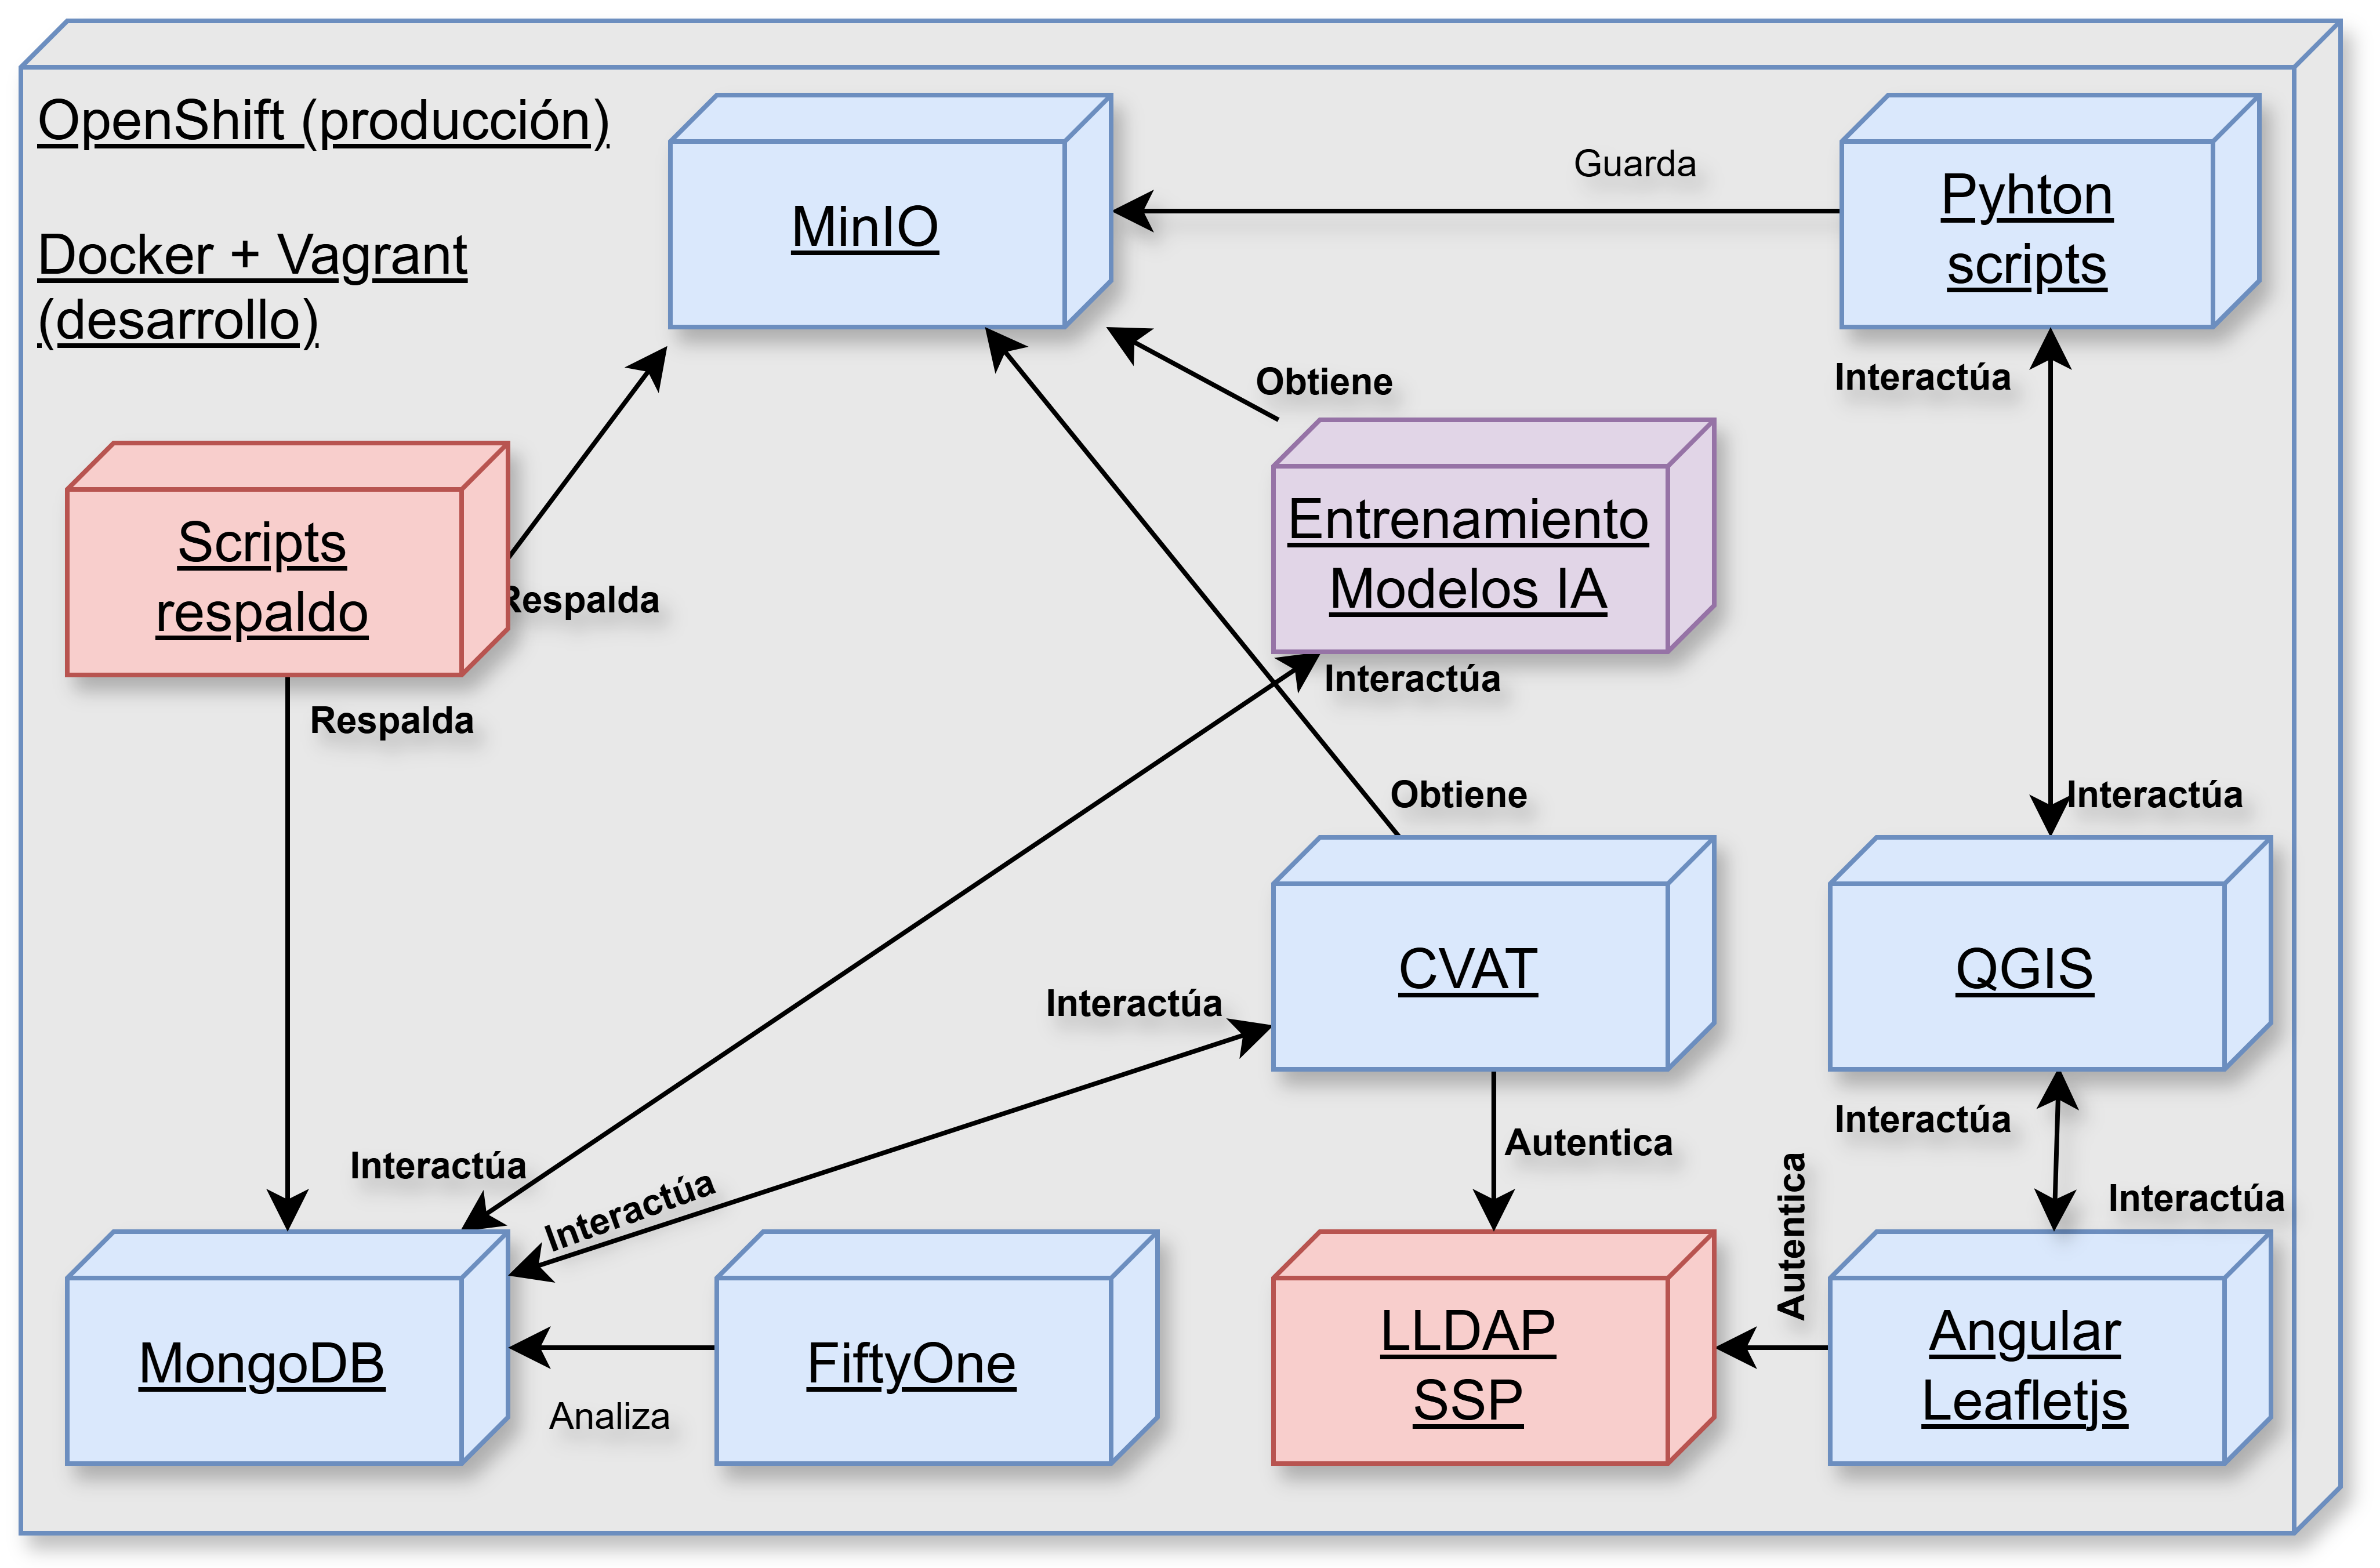
\includegraphics[scale=0.09]{./Figures/herramientas-plataforma.png}
  \caption{Diagrama de arquitectura del sistema de monitoreo.}
  \label{fig:infra-desarrollo}
\end{figure}

Otro usuario desarrollador puede tener el ambiente directamente desde su máquina, simplemente clonando el repositorio \citep{bruno_masoller_brunomaso1uba-ceia_nodate} mediante \textit{Git} y luego utilizar herramientas como \textit{Visual Studio Code} \citep{microsoft_documentation_nodate} para importar el proyecto.

La estructura de directorios para el ambiente de desarrollo del trabajo fue la siguiente:

% \begin{lstlisting}[label=cod:vControl,caption=Estructura de directorios utilizada.]  % Start your code-block
%
%   desarrollo/
%     |-- cvat/
%     |-- entrypoint/
%     |-- fiftyone/
%     |-- landing-page/
%     |-- ldap/
%     |-- ldap-self-service-password/
%     |-- minio/
%     |-- mongo/
%     |-- vagrant-scripts/
%     |-- mini-apps/
%     |-- readme.md
%     `-- Vagrantfile
%
% \end{lstlisting}

% \usepackage{alltt}
% \begin{alltt}
%
%   desarrollo/
%   ├── cvat/
%   ├── entrypoint/
%   ├── fiftyone/
%   ├── landing-page/
%   ├── ldap/
%   ├── ldap-self-service-password/
%   ├── minio/
%   ├── mongo/
%   ├── vagrant-scripts/
%   ├── mini-apps/
%   ├── readme.md
%   └── Vagrantfile
%
% \end{alltt}

\begin{lstlisting}[label=cod:vControl,caption=Estructura de directorios utilizada., literate={├}{{\textSFviii}}1 {─}{{\textSFx}}1 {└}{{\textSFii}}1 {│}{{\textSFxi}}1]  % Start your code-block

  desarrollo/
  ├── cvat/
  ├── entrypoint/
  ├── fiftyone/
  ├── landing-page/
  ├── ldap/
  ├── ldap-self-service-password/
  ├── minio/
  ├── mongo/
  ├── vagrant-scripts/
  ├── mini-apps/
  ├── readme.md
  └── Vagrantfile

\end{lstlisting}

La estructura de directorios está organizada de manera tal de que cada directorio representa un módulo del sistema, con su herramienta o conjunto de herramientas que implementa dicha funcionalidad. Estos directorios o módulos luego se pueden adaptar a otros administradores, como en el caso del módulo de seguridad que usualmente es administrado por el equipo de seguridad de la IM.

En ingeniería de software es importante asegurar la reproducibilidad de los ambientes de trabajo. Una de las herramientas utilizadas para asegurar esto es \textit{Docker}, que permite crear contenedores que encapsulan una aplicación y sus dependencias. Esto asegura un entorno de ejecución uniforme y reproducible en diferentes sistemas. Para la orquestación de múltiples contenedores utilizó \textit{Docker Compose}, que permite simular entornos complejos en donde interactúan varias aplicaciones.

Cada directorio tiene su propio archivo de \textit{Docker Compose} que habilita el despliegue de las herramientas del módulo. Esto permite que cada módulo pueda ser desarrollado y probado de manera independiente (con sus debidos \textit{stubs} \citep{wikipedia_talon_2025} o \textit{mocks} \citep{wikipedia_objeto_2024}), lo que facilita la integración y prueba del sistema completo. Estos archivos de configuración pueden ser adaptados a distintas situaciones. Por ejemplo, el archivo \textit{docker-compose.yml} de \textit{MinIO} fue adaptado para que si no existe el \textit{bucket} llamado "picudo-rojo-bucket", lo cree automáticamente, como se puede observar en el siguiente fragmento de código extraído de dicho archivo:

\begin{lstlisting}[label=cod:minio-mc,caption=Configuración del servicio MinIO Client (mc).]  % Start your code-block
  
  mc:
    image: minio/mc
    depends_on:
      - minio
    environment:
      - MINIO_ROOT_USER=${MINIO_ROOT_USER}
      - MINIO_ROOT_PASSWORD=${MINIO_ROOT_PASSWORD}
      - MINIO_INITIAL_BUCKET=${MINIO_INITIAL_BUCKET}
    entrypoint: >
      /bin/sh -c "
      until (/usr/bin/mc alias set myminio http://minio:9000 $MINIO_ROOT_USER $MINIO_ROOT_PASSWORD) do sleep 1; done;
      /usr/bin/mc mb myminio/${MINIO_INITIAL_BUCKET};
      /usr/bin/mc policy set public myminio/${MINIO_INITIAL_BUCKET};
      exit 0;
      "
    networks: *default-network
    
\end{lstlisting}

Este fragmento también evidencia que cada módulo tiene sus variables de entorno definidos como archivos \textit{.env} su directorio raíz. Esto permite separar la configuración de los distintos ambientas para cada  módulo. En este sentido, permite la fácil transición entre el ambiente de desarrollo y el ambiente de producción.

Aunque Docker permiten crear contenedores que emulan el ambiente de producción, no es suficiente para asegurar la reproducibilidad del ambiente de desarrollo. Esto se debe a que Docker se ejecuta sobre una plataforma, que puede ser diferente en cada máquina. Por lo tanto, es necesario utilizar una herramienta que permita crear y gestionar la infraestructura de soporte de manera uniforme y reproducible. Para esto se utilizó \textit{Vagrant} que administra máquinas virtuales de manera sencilla y reproducible.

Vagrant permite crear una (o varias) máquinas virtuales que emulan el ambiente de producción, inclusive con la misma versión del sistema operativo que se utiliza en el ambiente real (OpenShift). Se maneja con un archivo de configuración llamado (\textit{Vagrantfile}) que habilita la definición la configuración de la máquina virtual como \textit{infrastructure as a code}. Esto implica la posibilidad de definir parámetros como la cantidad de memoria, el sistema operativo o las aplicaciones a instalar. Se puede utilizar una imagen de un sistema operativo ya configurado o crear una desde cero. En este caso se utilizó una imagen de Ubuntu 24.04 LTS \citep{progress_chefs_bento_bentoubuntu-2404_nodate}, del repositorio oficial de \textit{Vagrant} \citep{hashicorp_hashicorp_nodate}, que incluye la mayoría de las herramientas necesarias para el desarrollo y despliegue del sistema. Esta imagen se puede utilizar en cualquier máquina que tenga instalado \textit{Vagrant} y \textit{VirtualBox} \citep{wikipedia_virtualbox_2025} (también se pueden utilizar otros software de virtualización, como lo es \textit{Hyper-V} \citep{meaghanlewis_informacion_2025} o \textit{VMWare} \citep{wikipedia_vmware_2025}), por lo que si otro desarrollador se incorpora al proyecto, puede utilizar la misma imagen y tener el mismo ambiente de desarrollo. Esto asegura que el sistema funcione de la misma manera en diferentes máquinas y evita problemas de compatibilidad entre diferentes versiones de software.

Para este trabajo, se utilizó el siguiente \textit{Vagrantfile}:

\begin{lstlisting}[label=cod:vagrantfile,caption=Configuración de Vagrant.]  % Start your code-block  
  
  Vagrant.configure("2") do |config|
    config.vm.box = "bento/ubuntu-24.04"
    config.vm.box_version = "202502.21.0"
    
    config.vm.network "public_network",
      bridge: "Intel(R) Wi-Fi 6E AX211 160MHz",
      use_dhcp_assigned_default_route: true  # Prioriza esta interfaz
  
    config.vm.disk :disk, size: "100GB", primary: true
  
    config.vm.provider "virtualbox" do |vb|
      vb.cpus = 8
      vb.memory = "32768"
      
      vb.customize ["modifyvm", :id, "--nic1", "nat"]
      vb.customize ["modifyvm", :id, "--nicpromisc1", "deny"] 
    end
  
    config.vm.provision "setup-vm-network", type: "shell", path: "vagrant-scripts/01-setup-network.sh"
    config.vm.provision "install-dependencies", type: "shell", path: "vagrant-scripts/02-install-dependencies.sh"
    config.vm.provision "setup-firewall", type: "shell", path: "vagrant-scripts/03-configure-firewall.sh"
    config.vm.provision "start-web-server", type: "shell", path: "vagrant-scripts/04-start-services.sh", run: "never" (*@\label{line:startwebserver}@*)
  end

\end{lstlisting}

Vagrant también permite aprovisionar \textit{scripts} de configuración a las máquinas virtuales. Éstos pueden ejecutarse al iniciar estas máquinas, lo que permite instalar y configurar las aplicaciones necesarias para el ambiente de desarrollo, pero también para el ambiente de producción. Se puede ejemplificar uno de estos aprovisionamientos en el script \ref{cod:vagrantfile} en la linea \ref{line:startwebserver}. En este caso, se utilizaron cuatro scripts de aprovisionamientos, en donde el último se encarga de iniciar los servicios dentro de cada módulo (usualmente se ejecuta mediante un script de shell el comando \textit{docker compose up}). Estos scripts se encuentran en el directorio \textit{vagrant-scripts}.

Una vez que se ejecuta el comando \textit{vagrant up}, se crea la máquina virtual (si ya no fue creada) y se ejecutan los scripts de aprovisionamiento, lo que permite obtener el ambiente de desarrollo en pocos minutos. Entre los servicios que se inician se encuentran:

\begin{itemize}
  \item \textit{MongoDB}: herramienta que implementa la base de datos, dentro del módulo de gestión de datos, que permite almacenar metadatos de las imágenes ortorectificadas y los resultados de los modelos.
  \item \textit{MinIO}: herramienta que un repositorio de objetos dentro del módulo con el mismo nombre que almacena las imágenes generadas por los drones y aviones.
  \item \textit{CVAT}: herramienta de etiquetado de imágenes, perteneciente al módulo de datos, que se utiliza para etiquetar las imágenes almacenadas en el repositorio de objetos.
  \item \textit{FiftyOne}: herramienta de análisis, organización, visualización y generación de informes sobre los datos. Pertenece al módulo de calidad de datos.
  \item \textit{LLDAP}: herramienta de gestión de usuarios y permisos, utilizada para administrar la seguridad del sistema. Permite gestionar el acceso a la información sensible de manera sencilla y eficiente. Integrada en el módulo de seguridad.
  \item \textit{LDAP Self Service Password}: herramienta de gestión de contraseñas, utilizada para que los usuarios manejen sus credenciales. Se integra con LLDAP y pertenece al mismo módulo.
  \item \textit{Landing Page}: conjunto de herramientas basadas en tecnologías de desarrollo web (HTML, CSS, Javascript) que brindan información sobre el proyecto. Es la cara visible del sistema desde internet. Se asocia con el módulo de aplicaciones web.
  \item \textit{Mini-apps}: son scripts que ejecutan varias tareas, como por ejemplo, obtener las imágenes desde el SIG de la IM. Pertenece al módulo de \textit{mini-apps}.
  \item \textit{Entrypoint}: es un proxy reverso que expone el ambiente de desarrollo a internet para su fácil acceso. Pertenece al módulo de aplicaciones web.
\end{itemize}

% Poner un esquema de flujo (caso de uso) de la plataforma, mostrando los módulos y su interacción.
% Hablar un poco más sobre cada módulo y como se desliega.
% Mostrar alguna imagen del acceso desde internet a la plataforma, como por ejemplo el acceso a la landing page o al sistema de etiquetado de imágenes.
% Hablar de los problemas encontrados durante el despliege de la plataforma. Porque se eligió cada herramienta. Hablar del tema de CVAT vs Label Studio.

%----------------------------------------------------------------------------------------
%	SECTION 3
%----------------------------------------------------------------------------------------

\section{Proceso de etiquetado de datos}
\label{sec:etiquetado}

% Hablar de los tipos de usuarios, las pruebas que se realizaron -de control, no en profundidad- y las jornadas de etiquetado.
% También como se midió el progreso. Hablar del enfoque que se tomó (recortar las imágenes).
% Mostrar algunos de los etiquetados finales.

%----------------------------------------------------------------------------------------
%	SECTION 4
%----------------------------------------------------------------------------------------

\section{Entrenamiento de los modelos}
\label{sec:entrenamiento}

% Hablar del proceso de entrenamiento de los modelos.

%----------------------------------------------------------------------------------------
%	SECTION 5
%----------------------------------------------------------------------------------------

\section{Despliegue de los modelos}
\label{sec:despliegue_modelos}

% Hablar del proceso de despliegue de los modelos.
% Hablar de la integración con el resto de la plataforma.
% Hablar de las herramientas utilizadas para el despliegue de los modelos.
% Hablar de los problemas encontrados y como se resolvieron.
